\section{A Test on the Database}
\label{sec:test}
In this chapter, we present a digit recognition system on the Poissonian subset as an example use of the dataset.
Both the training and testing exploited the Poinssonian presentation of the digits.
The network was trained online with STDP learning rule.
The performance of the model was evaluated with both software simulation (on NEST~\cite{gewaltig2007nest}) and hardware implementation (on SpiNNaker). 
%\subsection{Description of the data used}
\subsection{Training}
There are two layers in the neural network model.
And 28$\times$28 input neurons fully connected to 100 output neurons.
Each output neuron represented a trained template of a digit.
Thus there were 10 templates for each digit.
The firing rate of the input neurons were assigned linearly according to their intensities and normalised with a total firing rate of 2000~$Hz$.
The training set of 60000 hand written digits were firstly classified into 100 classes, 10 classes per digit, using K-means clusters.
Every image was presented 300~$ms$ during training and at the same time a teaching signal of 50~$Hz$ was conveyed to the responding output neuron (1 out of 100) to trigger the learning.
The model utilised Leaky-Integrate-and-Fire (LIF) neurons, and the parameters were all with biological means, see the listed values in Table~.
The trained weights were plotted in align with the input image size in Fig~\ref{Fig:weight}.
\begin{figure}[hbt!]
	\centering
	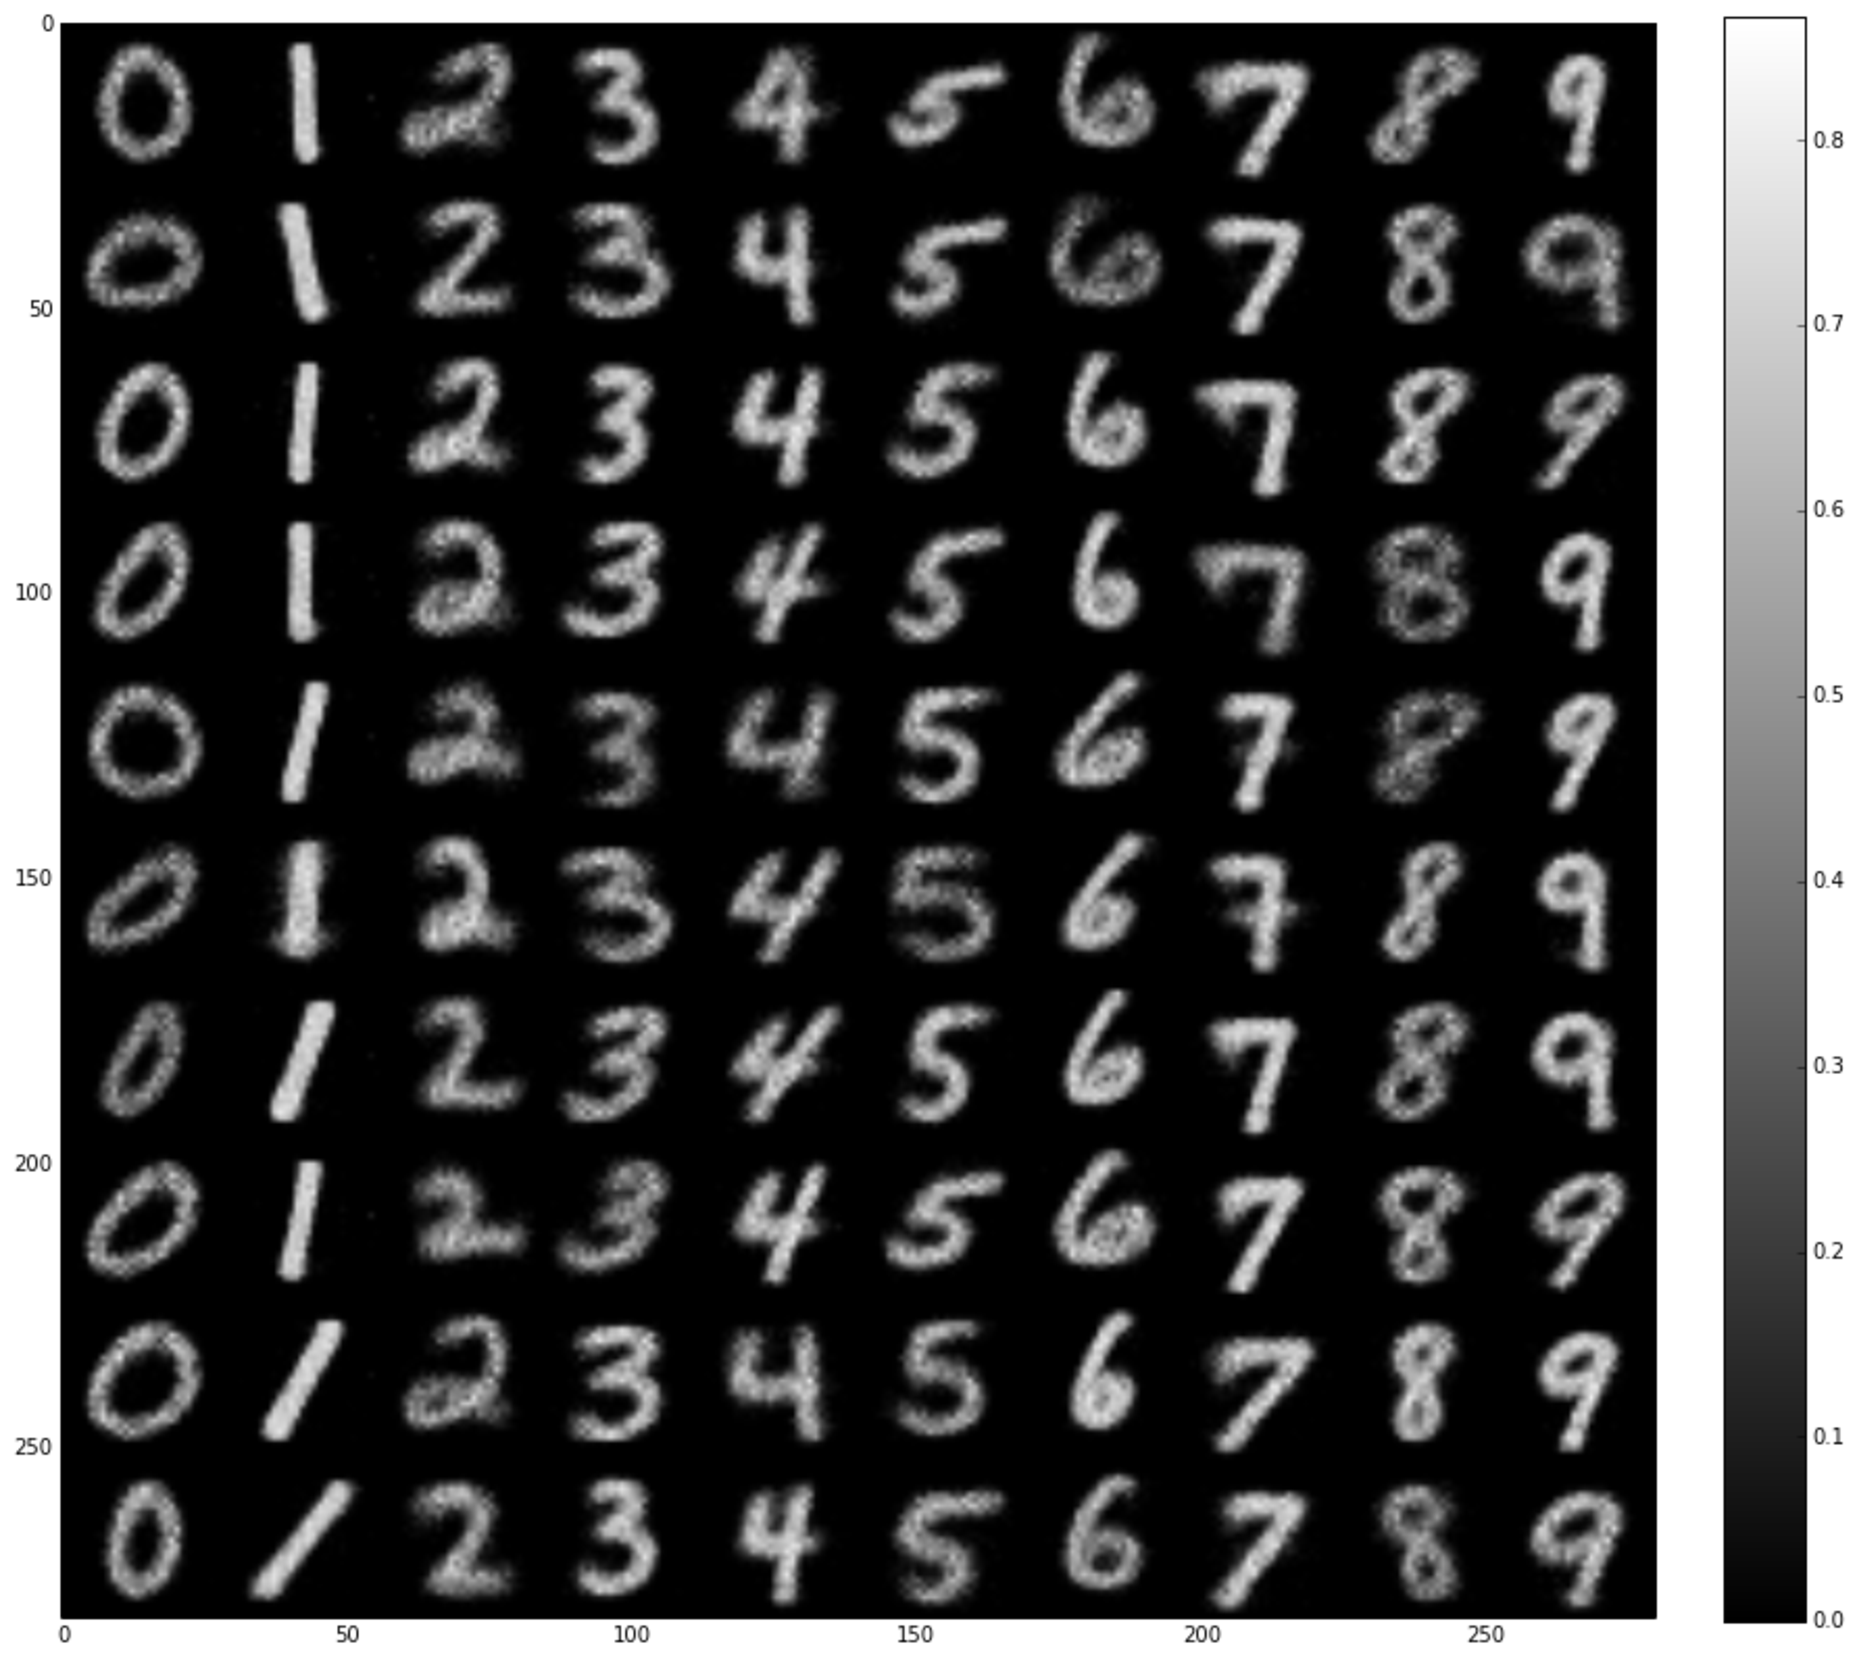
\includegraphics[width=0.48\textwidth]{images/weight.pdf}
	\caption{Trained weights of the synapses from input layer to output neurons.}
	\label{Fig:weight}
\end{figure}  
 
\subsection{Testing}
The weights were normalised after training and applied to the same network.
And weak weights (=0) were set to inhibitory connections with an identical strength.
The output neurons inhibited all the other neurons as a winner take all circuit.
Every testing image was presented 1 second to the network, and the output neuron with the highest firing rate won.
The accuracy of the recognition reached 83.14\%.
The recording of the output neurons of a test sequence of digits (4, 1, 1, 0, 9, 3, 1, 9, 4, 6) was shown in the raster plot (Fig~\ref{Fig:output}).
\begin{figure}[hbt!]
	\centering
	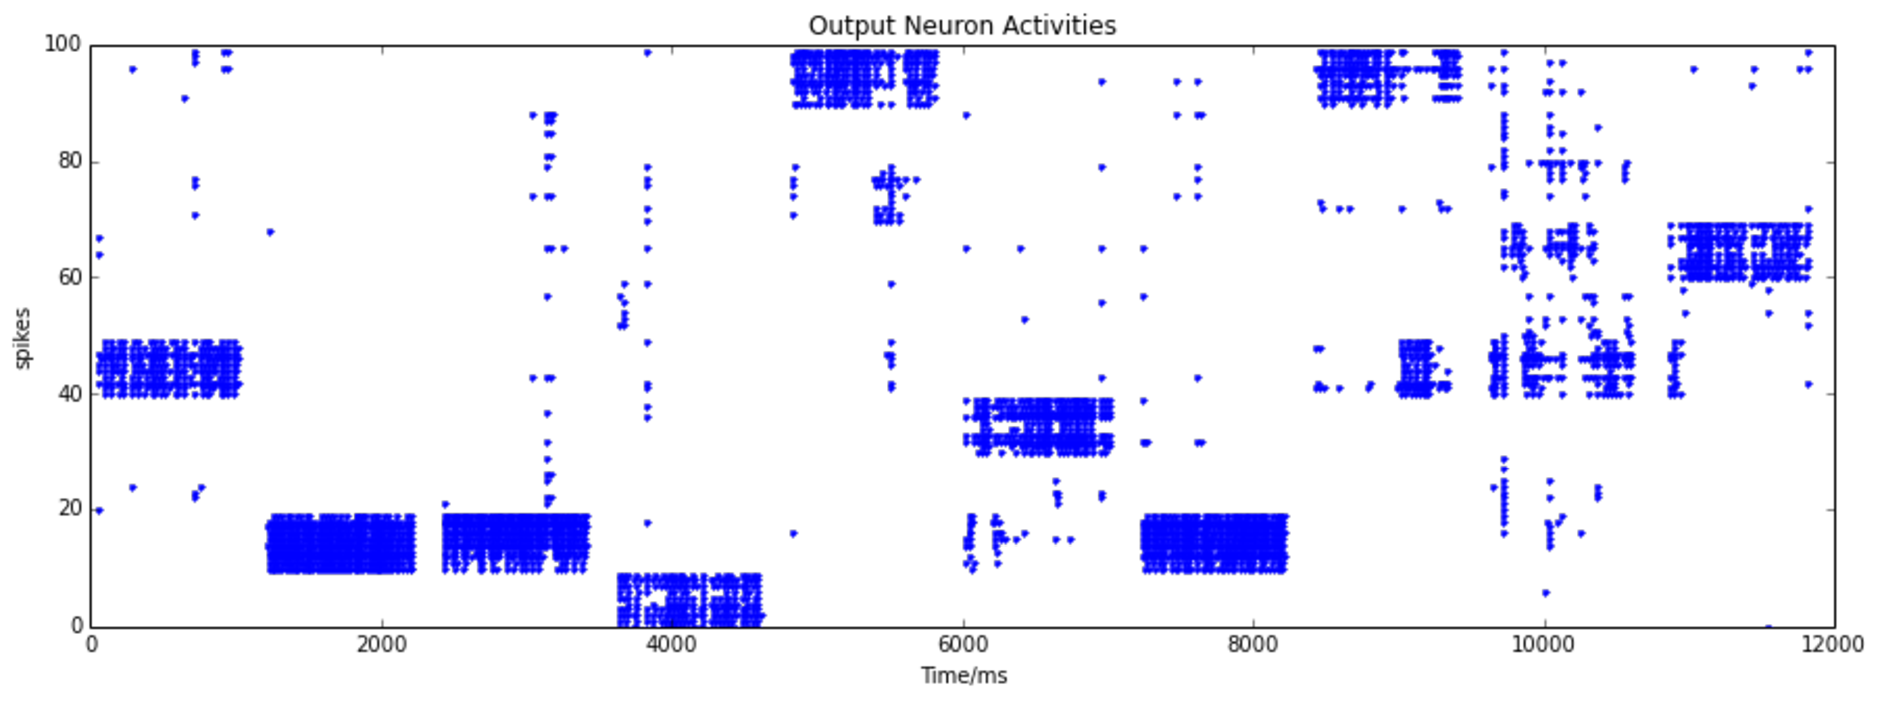
\includegraphics[width=0.48\textwidth]{images/test300-301.pdf}
	\caption{A raster plot of test of a digits sequence.}
	\label{Fig:output}
\end{figure} 
\subsection{Evaluation}

	